\section{Fine Control Strategy: Visual Servoing}
\label{sec:fine_control}
While the global perception system (RealSense) provides coarse brick localization, it suffers from perspective occlusion and calibration inaccuracies at the millimeter scale. To achieve precise grasping, a "Fine Control" layer was developed for the AR4 robotic arm. This layer utilizes an \textbf{Eye-in-Hand} configuration with an ESP32-CAM and implements an Image-Based Visual Servoing (IBVS) controller.

The control strategy follows a \textbf{Global-to-Local Handoff} approach:
\begin{enumerate}
    \item \textbf{Coarse Alignment:} The global camera provides the brick pose, guiding the AR4 to an "Approach Point" ($\approx 15$ cm above the target).
    \item \textbf{Feature Handoff:} A Homography transformation maps the detected grasp point from the global view to the local eye-in-hand view, providing an initial search region.
    \item \textbf{Fine Servoing:} The IBVS controller takes over, using local camera feedback to minimize pixel error and achieve precise gripper alignment.
\end{enumerate}

\subsection{System Architecture Overview}

The complete visual servoing pipeline integrates perception, transformation logic, and control as illustrated in Figure~\ref{fig:vs_architecture}. The system operates in three primary stages:

\begin{figure}[H]
    \centering
    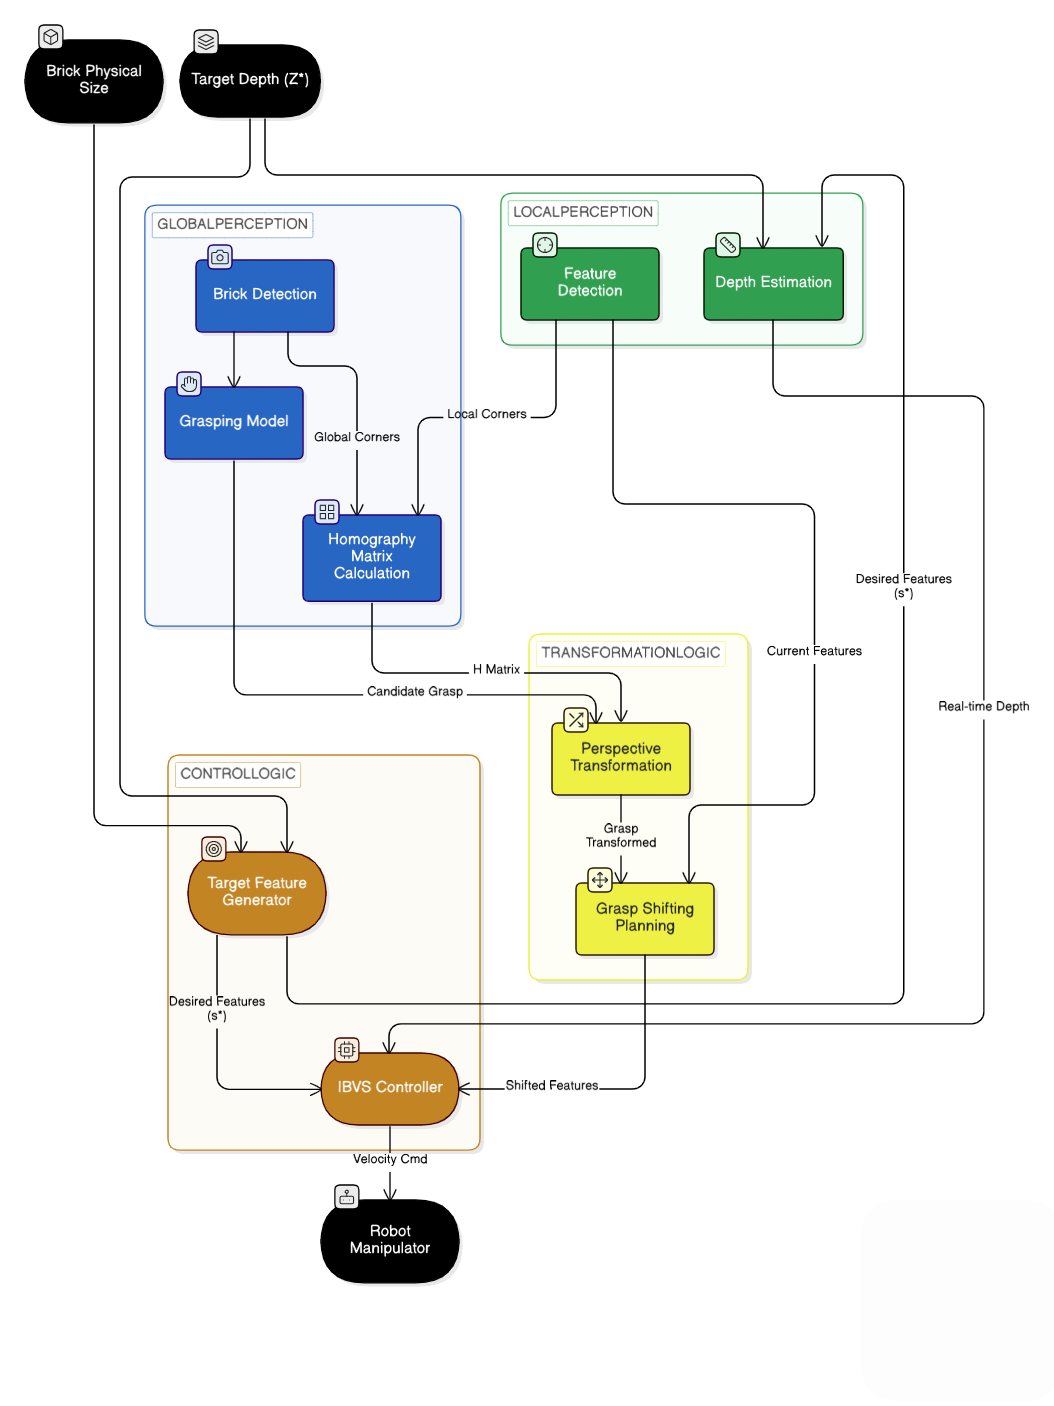
\includegraphics[width=1.0\textwidth]{Figures/chapter3/VISP/VisualServoDiagram.png}
    \caption{Complete visual servoing system architecture showing data flow from global perception through local feedback control. Two deep learning models extract object type and grasp point; these feed the homography calculation and target feature generation pipeline.}
    \label{fig:vs_architecture}
\end{figure}

\subsubsection{Global Perception Stage}
The global perception module executes on the RealSense camera, providing:
\begin{itemize}
    \item \textbf{Brick Detection Model:} Extracts the object type (I-brick, L-brick, T-brick) and computes oriented bounding boxes of all visible bricks.
    \item \textbf{Grasping Model:} Predicts the optimal grasp point (center of the graspable face) for each detected brick.
    \item \textbf{Homography Initialization:} Uses the detected brick corners and estimated grasp point as reference data for the global-to-local transformation.
\end{itemize}

\subsubsection{Transformation Logic Stage}
This stage bridges the two camera views through projective geometry:
\begin{itemize}
    \item \textbf{Perspective Transformation:} Computes the homography matrix $H$ relating global and local image coordinates.
    \item \textbf{Grasp Point Projection:} Transfers the global grasp prediction into the local camera frame.
    \item \textbf{Grasp Shifting Planning:} Adjusts feature reference points to account for grasp offset from the brick centroid.
\end{itemize}

\subsubsection{Local Control Stage}
The local perception and control modules execute on the host PC:
\begin{itemize}
    \item \textbf{Feature Detection:} Extracts the brick's corner features in real-time using color-based ROI tracking.
    \item \textbf{Depth Estimation:} Maintains an online estimate of the brick's distance from the camera.
    \item \textbf{Target Generation:} Creates desired feature references based on the brick type and grasp offset.
    \item \textbf{IBVS Control:} Computes velocity commands to minimize pixel error and achieve alignment.
\end{itemize}

\subsection{Local Perception Implementation}

\subsubsection{Fisheye Undistortion and Linear Space Projection}
The ESP32-CAM employs a $160^\circ$ wide-angle fisheye lens to maintain visibility of the brick during approach. However, the standard IBVS control law (Section~\ref{sec:ibvs_theory}) assumes linear (pinhole) projection. To maintain theoretical validity while exploiting the wide field of view, we employ a \textbf{rectification strategy}:

All raw images from the ESP32-CAM are mathematically undistorted using the camera intrinsic matrix $K$ and distortion coefficients $D$, obtained via checkerboard calibration:
\begin{equation}
    p_{linear} = \text{undistort}(p_{fisheye}, K, D)
\end{equation}

This transformation linearizes the projection in the central workspace region where grasping occurs, allowing standard Interaction Matrices to remain valid. The undistorted coordinates serve as inputs to all downstream modules.

\subsubsection{Corner-Based Feature Extraction}
Rather than relying on single-point features, we extract the \textbf{four corner points} of the brick's bounding rectangle. This representation provides:
\begin{itemize}
    \item Redundancy and robustness to partial occlusions or tracking failures
    \item Sufficient constraints for pose estimation and shape analysis
    \item Reliable depth cues via area-based approximations
\end{itemize}

The feature extraction pipeline proceeds as follows:


\begin{enumerate}
    \item \textbf{HSV Color Segmentation:} The undistorted image is converted to HSV color space and thresholded to isolate pixels matching the target brick color. HSV is chosen for its robustness to illumination variations compared to RGB space.
    
    \item \textbf{Morphological Processing:} To address the challenge of detecting L-shaped bricks whose two perpendicular edges may appear as disconnected components in the binary mask, we employ morphological \textbf{closing} (dilation followed by erosion). This operation bridges small gaps between the L-shaped legs without growing the overall contour, enabling robust detection of the complete brick boundary as a single connected component.
    
    \item \textbf{Geometric Analysis:} For each valid blob, we compute the bounding box orientation and corner points via minimum area rectangle fitting. The corner points are sorted in counter-clockwise order relative to their centroid, ensuring consistent feature correspondence.
    
    \item \textbf{ROI-Based Tracking:} To maintain tracking stability and reduce computational load, the system maintains a Region of Interest (ROI) around the predicted brick location. Tracking searches within this adaptive ROI first; if no valid target is found, a full-image search is performed.
    
    \item \textbf{Stability Filtering:} Detected features are validated against previous detections using two criteria:
    \begin{itemize}
        \item \textbf{Position Continuity:} The centroid displacement from the previous frame must be less than a maximum jump distance (default: 30 pixels).
        \item \textbf{Area Consistency:} The relative area change from the previous frame must be less than a maximum ratio (default: 40\%).
    \end{itemize}
    
    If validation fails, the detection is rejected and the previous feature state is retained, preventing sudden spurious jumps. After a configurable number of rejections (default: 10), the system re-initializes tracking on a new object.
\end{enumerate}

All corner features are published in \textbf{linear (undistorted) space} to ensure consistency across the pipeline. This is critical for accurate homography computation and Jacobian matrix evaluation.

\subsection{Depth Estimation via Area-Based Scaling}

\subsubsection{Monocular Depth Challenge}
The Interaction Matrix (Image Jacobian) derived in Section~\ref{sec:ibvs_theory} depends explicitly on the depth $Z$ of feature points relative to the camera frame. With a monocular camera, $Z$ is inherently unobservable from image data alone. However, for planar objects like bricks at a known working height, we can exploit geometric relationships to estimate depth online.

\subsubsection{Area-Based Depth Approximation}
For a planar rectangular object observed under perspective projection, the projected area $A$ is inversely proportional to the squared distance $Z$:
\begin{equation}
    A \propto \frac{1}{Z^2}
\end{equation}

By establishing a calibration at a known reference depth $Z^*$ with corresponding reference area $A^*$, we can estimate the current depth using the area ratio:
\begin{equation}
    \hat{Z} = Z^* \sqrt{\frac{A^*}{A_{current}}}
    \label{eq:area_depth}
\end{equation}

This approximation holds well for objects remaining approximately parallel to the image plane (which is enforced by the visual servoing control law).

\subsubsection{Implementation Details}
The depth estimator node maintains the following state:

\begin{itemize}
    \item \textbf{Target Depth $Z^*$:} The desired grasping distance, typically 0.2 m. This parameter is constant across a mission.
    
    \item \textbf{Desired Feature Area $A^*$:} Updated dynamically whenever a new desired feature set is generated by the target generator. This allows seamless transitions between brick types and grasp offsets.
    
    \item \textbf{Current Area $A_{current}$:} Computed from the four corner features using the shoelace formula:
    \begin{equation}
        A = \frac{1}{2} \left| \sum_{i=0}^{3} (x_i y_{i+1} - x_{i+1} y_i) \right|
    \end{equation}
    where indices wrap around modulo 4.
\end{itemize}

The raw depth estimate from Equation~\ref{eq:area_depth} is smoothed with a first-order low-pass filter to reduce jitter:
\begin{equation}
    Z_{filtered}(t) = \alpha \hat{Z}(t) + (1 - \alpha) Z_{filtered}(t-1)
\end{equation}

where $\alpha$ is the smoothing factor (default: 0.2). The filtered depth is published at 10 Hz and consumed by the IBVS controller.

\subsection{Global-to-Local Handoff via Homography}

The global perception system detects bricks and estimates grasp points in the RealSense camera frame. To initialize visual servoing in the ESP32-CAM frame, we must establish a geometric correspondence between these two views.

\subsubsection{Homography Matrix Computation}
A homography matrix $H$ represents the projective transformation between two planes. In our setup, $H$ maps pixel coordinates from the global (RealSense) view to the local (ESP32-CAM) view, assuming both cameras observe the same planar brick surface.

To compute $H$ robustly:

\begin{enumerate}
    \item \textbf{Feature Detection in Both Views:} Extract the four corner points of detected bricks in both camera frames. Importantly, these corners must be in linear (undistorted) space for the homography to remain valid.
    
    \item \textbf{Geometric Matching:} Match bricks detected in the global view with those in the local view using aspect ratio constraints. The ratio of short-to-long edges is computed for each detection:
    \begin{equation}
        r = \frac{\text{short edge}}{\text{long edge}}
    \end{equation}
    Two detections are matched if $|r_{global} - r_{local}| < \epsilon$, where $\epsilon = 0.2$ is the tolerance threshold. This constraint ensures robust correspondence despite viewpoint differences and small perspective changes.
    
    \item \textbf{RANSAC Homography Estimation:} The matched corner pairs are fed into the RANSAC algorithm to compute a robust homography matrix:
    \begin{equation}
        \text{corners}_{local} = H \text{corners}_{global}
    \end{equation}
    RANSAC iteratively:
    \begin{itemize}
        \item Selects random subsets of 4 point correspondences
        \item Computes a candidate homography matrix from each subset
        \item Projects all global points using the candidate $H$ and counts inliers (points with reprojection error $< 5$ pixels)
        \item Retains the homography with the best inlier support
    \end{itemize}
    
    This robustness is critical for handling detection noise and occlusions.
    
    \item \textbf{Grasp Point Projection:} Once $H$ is computed and validated, the grasp point detected in the global view is projected to the local view:
    \begin{equation}
        p_{local} = H \cdot p_{global}
    \end{equation}
    This projected point serves as the initial target location for the grasp shifting planning module.
\end{enumerate}

\subsubsection{Sticky Tracking Strategy}
Once a homography is established, it remains valid as long as the same brick is tracked. The system employs a \textbf{sticky tracking} mechanism:

\begin{itemize}
    \item \textbf{Initialization Phase:} When a new mission begins (brick type changes), the homography is reset. The system enters search mode, scanning incoming detections from both cameras until a geometric match is found.
    
    \item \textbf{Tracking Phase:} Once a match is found and $H$ is computed, the system "sticks" to that correspondence. Subsequent detections are matched to the previous brick by minimizing centroid distance, even if geometric ratios vary slightly due to perspective changes.
    
    \item \textbf{Re-initialization:} If tracking is lost (no detections in the local view for an extended period), the homography is cleared and the system returns to search mode.
\end{itemize}

\subsection{Grasp Point Adaptation via Shifting Planning}

The grasp point detected by the grasping model is not necessarily the brick's centroid. Instead, it represents the optimal location on the brick's face for the gripper to approach. However, visual servoing with corner-based features naturally drives the brick's centroid to the image center.

To resolve this mismatch, we employ a \textbf{grasp shifting} strategy that adjusts the feature reference set based on the offset between the centroid and grasp point.

\subsubsection{Grasp Offset Computation}
At the moment a new grasp point is selected:

\begin{enumerate}
    \item \textbf{Reference Latch:} Store the current brick's corner features and the projected grasp point as reference data.
    
    \item \textbf{Shift Vector Calculation:} As the brick moves in the image, compute the transformation of the brick's shape using homography:
    \begin{equation}
        H_{local} = \text{findHomography}(\text{ref\_corners}, \text{curr\_corners}, \text{RANSAC})
    \end{equation}
    
    Apply this transformation to the reference grasp point to track how it moves as the brick deforms/rotates:
    \begin{equation}
        p_{grasp,current} = H_{local} \cdot p_{grasp,reference}
    \end{equation}
    
    \item \textbf{Adaptive Feature Offset:} Compute the shift vector from the current centroid to the grasp point:
    \begin{equation}
        \Delta p = p_{grasp,current} - \text{centroid}_{current}
    \end{equation}
    
    Apply this offset to all corner features:
    \begin{equation}
        s_{shifted} = s_{current} + \Delta p
    \end{equation}
    
    The shifted features are fed to the IBVS controller instead of the raw features. This tricks the controller into aligning the brick's centroid with the grasp point.
\end{enumerate}

\subsubsection{Benefits of Shifting Strategy}
\begin{itemize}
    \item Allows visual servoing to guide the gripper to a precise offset on the brick, not just the centroid.
    \item Compensates for changes in brick pose and shape as it is manipulated.
    \item Maintains control stability by working with the same robust corner features.
\end{itemize}

\subsection{Target Feature Generation}

Before visual servoing can begin, desired feature locations $s^*$ must be computed based on the brick's physical dimensions and the desired grasping geometry.

\subsubsection{Brick Model and Dimensions}
The system supports three brick types, each with known physical dimensions:

\begin{table}[H]
    \centering
    \begin{tabular}{|l|c|c|}
        \hline
        \textbf{Brick Type} & \textbf{Length (m)} & \textbf{Width (m)} \\
        \hline
        I-Brick & 0.058 & 0.030 \\
        L-Brick & 0.060 & 0.060 \\
        T-Brick & 0.090 & 0.030 \\
        \hline
    \end{tabular}
    \caption{LEGO brick physical dimensions used for target feature generation.}
\end{table}

\subsubsection{Desired Feature Projection}
Given a brick type with dimensions $(L, W)$ and a target depth $Z^*$:

\begin{enumerate}
    \item \textbf{3D Corner Generation:} Generate the brick's four corner points in 3D (world frame):
    \begin{equation}
        \text{corners}_{3D} = \begin{bmatrix}
            -L/2 & -W/2 & 0 \\
            L/2 & -W/2 & 0 \\
            L/2 & W/2 & 0 \\
            -L/2 & W/2 & 0
        \end{bmatrix} + \begin{bmatrix} 0 & 0 & Z^* \end{bmatrix}
    \end{equation}
    
    \item \textbf{Rotation and Offset Strategy:} Rather than using four discrete rotation angles (0°, 90°, 180°, 270°), the system employs an efficient two-rotation strategy combined with adaptive offset application to avoid expensive 180° rotations. The brick's orientation is determined by the shift vector $\Delta p$ from the grasp shifting module:
    \begin{equation}
        \text{offset}_{\text{rot}} = \begin{cases}
            \pi/2 & \text{if } |\Delta x| > |\Delta y| \text{ (horizontal grasp)} \\
            0 & \text{if } |\Delta y| > |\Delta x| \text{ (vertical grasp)}
        \end{cases}
    \end{equation}
    
    The direction of the grasp (left/right for horizontal, up/down for vertical) is encoded as an \textbf{offset sign} that determines whether the hand-eye offset is \textit{added} or \textit{subtracted}:
    \begin{equation}
        \text{offset}_{\text{sign}} = \begin{cases}
            -1 & \text{if grasp points left or up} \\
            +1 & \text{if grasp points right or down}
        \end{cases}
    \end{equation}
    
    This approach eliminates 180° rotations while maintaining correct target placement through offset adjustment.
    
    \item \textbf{3D Rotation and Offset Application:} Apply the computed rotation and offset to the corner positions:
    \begin{equation}
        \text{corners}_{offset} = R(\text{offset}_{\text{rot}}) \cdot \text{corners}_{3D}^T + \begin{bmatrix} 0 \\ \text{offset}_{\text{sign}} \cdot d_{hand-eye} \\ 0 \end{bmatrix}
    \end{equation}
    
    where $d_{hand-eye}$ is the physical offset between the camera and gripper center.
    
    \item \textbf{Perspective Projection:} Project the offset 3D corners onto the image plane using the camera intrinsic matrix $K$:
    \begin{equation}
        p_{pixel} = K \cdot \frac{\text{corners}_{offset}}{Z^*}
    \end{equation}
    
    The resulting pixel coordinates form the desired feature vector $s^*$ fed to the IBVS controller.
\end{enumerate}

\subsubsection{Caching and Stability}
The desired features are computed once per mission when the brick type is known. They are then cached and reused until a new brick type is selected. This ensures:
\begin{itemize}
    \item Consistent target throughout the control task
    \item Reduced computational overhead (no re-computation during control)
    \item Predictable control behavior
\end{itemize}

\subsection{IBVS Controller Implementation}

The Image-Based Visual Servoing controller is the final module that transforms error signals into robot velocity commands.

\subsubsection{Feature Error Definition}
The controller minimizes the error between current and desired features:
\begin{equation}
    e(t) = s(t) - s^*(t)
\end{equation}

where $s = [u_1, v_1, u_2, v_2, u_3, v_3, u_4, v_4]^T$ represents the pixel coordinates of the four brick corner features.

\subsubsection{Interaction Matrix and Control Law}
For each feature point $(u_i, v_i)$ at depth $Z$, the Interaction Matrix (Image Jacobian) is:
\begin{equation}
    L_{s,i} = \begin{bmatrix}
        -\frac{1}{Z} & 0 & \frac{u_i}{Z} & u_i v_i & -(1+u_i^2) & v_i \\
        0 & -\frac{1}{Z} & \frac{v_i}{Z} & 1+v_i^2 & -u_i v_i & -u_i
    \end{bmatrix}
\end{equation}

For four corner features, the stacked Interaction Matrix is $8 \times 6$, providing redundancy. The control law is:
\begin{equation}
    v_c = -\lambda L_s^+ e
\end{equation}

where $L_s^+$ is the Moore-Penrose pseudo-inverse and $\lambda$ is the control gain.

\subsubsection{Hybrid Control Strategy}
The controller implements a \textbf{hybrid approach} that decouples XY (image plane) and Z (depth) control:

\begin{enumerate}
    \item \textbf{XY-Plane Control (Centroid Alignment):} Uses a PID controller on the error between desired and current centroid positions:
    \begin{equation}
        v_x = -k_p e_u - k_i \sum e_u - k_d \frac{de_u}{dt}
    \end{equation}
    \begin{equation}
        v_y = -k_p e_v - k_i \sum e_v - k_d \frac{de_v}{dt}
    \end{equation}
    
    where $k_p$, $k_i$, $k_d$ are proportional, integral, and derivative gains (tuned experimentally).
    
    \item \textbf{Z-Axis Control (Area-Based Depth):} Uses an area-based controller to regulate the brick size:
    \begin{equation}
        \text{area\_error} = \frac{A^* - A_{current}}{A^*}
    \end{equation}
    
    The Z-velocity follows an adaptive gain law:
    \begin{equation}
        v_z = \text{area\_error} \cdot \left( \lambda_{z,0} + (\lambda_{z,\infty} - \lambda_{z,0}) e^{-\beta_z |\text{area\_error}|} \right)
    \end{equation}
    
    This gain scheduling ensures aggressive approach when far from target and gentle deceleration as the brick approaches the desired size.
    
    \item \textbf{YAW Control (Rotation):} Uses ViSP's computed rotation component from the full Interaction Matrix:
    \begin{equation}
        \omega_z = \text{gain}_{yaw} \cdot v_{visp,z}
    \end{equation}
    
    where $v_{visp,z}$ is the rotation component of the ViSP solver.
\end{enumerate}

\subsubsection{Acceleration Ramping and Saturation}
To ensure smooth acceleration and respect physical robot limits, velocity commands are subject to:

\begin{enumerate}
    \item \textbf{Acceleration Limiting:}
    \begin{equation}
        v_{out}(t) = v_{prev}(t-1) + \text{clamp}\left( v_{target} - v_{prev}(t-1), -a_{max} \Delta t, a_{max} \Delta t \right)
    \end{equation}
    
    where $a_{max}$ is the maximum acceleration (default: 0.25 m/s² for linear, 1.5 rad/s² for angular).
    
    \item \textbf{Velocity Saturation:}
    \begin{equation}
        v_{final} = \text{clamp}(v_{out}, -v_{max}, v_{max})
    \end{equation}
    
    where $v_{max}$ is the maximum velocity (default: 0.15 m/s for linear, 0.5 rad/s for angular).
\end{enumerate}

\subsubsection{Latency Compensation}
The ESP32-CAM introduces WiFi transmission latency ($\approx 150$ ms). To mitigate oscillations caused by this delay, the proportional gain is set conservatively to $k_p = 0.0006$, with low integral gain to avoid aggressive responses to delayed feedback.

\subsubsection{Logging and Monitoring}
The controller logs performance metrics to a CSV file for offline analysis:
\begin{itemize}
    \item Timestamp and elapsed time
    \item Feature error norm
    \item Computed velocity commands $(v_x, v_y, v_z, \omega_z)$
    \item Current depth estimate $Z$
    \item Area error and other state variables
\end{itemize}

These logs enable post-hoc performance analysis and gain tuning iterations.
